\chapter{AtariEyes package}

\label{ch:atarieyes}

This chapter describes the software realized in this thesis, that we called
``AtariEyes''. Its purpose is both to implement the ideas that have been
presented in previous chapters and to generate the experiments shown
Chapter~\ref{ch:experiments}.

Apart from being a realization of the ideas proposed, this software has some
interesting qualities:
\begin{description}
	\item [Clarity] Every method and structure has been documented.
	\item [Efficiency] Thanks to an heavy use of parallel computing libraries,
		it benefits from GPU acceleration.
	\item [User friendly] The extensive command line interface allows to
		experiment with the package as it is, or, thanks to its modular design,
		individual structures can be reused in future developments.
\end{description}

Regarding its general functionality, through the commands provided, the user
can:
\begin{itemize}
	\item Choose any \emph{environment} from the Atari~2600 collection.
	\item Train a Deep Reinforcement Learning \emph{agent}. The algorithm is
		Double DQN and the agent's model can be either the original Atari model
		(Section~\ref{sec:model-atari}) or the restricted agent
		(Section~\ref{sec:model-atari-rb}).
	\item Train the \emph{feature extractor}, because it implements every model
		and algorithm presented in Chapter~\ref{ch:fluents}.
	\item \emph{Play}, \emph{visualize} and \emph{record} any of these
		agents while they interact with the environment.
\end{itemize}

This chapter is divided in two sections: Section~\ref{sec:how-to-use}
documents how the software can be used from a user perspective;
Section~\ref{sec:implementation} is a larger part that explains some of the
most interesting details about the implementation.
%While the former is really
%useful for an high-level overview, the latter highlights some interesting
%parts which may be useful also in future developments.


\section{How to use the software}

\label{sec:how-to-use}

\subsection{Tools and setup}

The software \texttt{AtariEyes} is a Python package. It is publicly available
at the GitHub repository:
\href{https://github.com/cipollone/atarieyes}{\texttt{cipollone/atarieyes}}.
It can be installed with the \texttt{pip} commandAs any other Python package,
we just need to point to this git repository. The installation
command is:
\begin{lstlisting}[style=bash]
pip install git+https://github.com/cipollone/atarieyes
\end{lstlisting}
This installs this package from the master branch. If we need to work on some
specific revision, for example on the \texttt{develop} branch, we can append
\verb!@develop! or any other commit to the previous address.

Dependencies are automatically installed by \texttt{pip}.  In Python, it is
common to run applications inside virtual environments. Just run this
installation command within a container to avoid dependency conflicts with
other applications. One rather particular dependency is TensorFlow, which is a
famous Machine Learning library that we use for parallel computing. Following
the instructions of the specific container application, we can reuse some
preexisting system installation, if we need. Currently, the supported version
is only 2.1, but future 2.x versions might also be compatible.

The package is written in Python~3 and the minimum version required for the
interpreter is 3.7. This requirement should be met by most modern operating
systems. If that's not the case, we suggest to use \texttt{pyenv}, which
allows environment-specific Python installations.

Once installed, we can use the \texttt{atarieyes} package. As we will see, we
often use this module through its command line interface. However, if we want
just to include some structures and algorithms in other applications, we can
\lstinline[style=inlinepy]|import atarieyes|, as usual. For development it may
be also useful to look at the source code. We can clone the repository:
\begin{lstlisting}[style=bash]
git clone https://github.com/cipollone/atarieyes.git
\end{lstlisting}
This is also useful if, for any reason, some updated dependency is no longer
compatible with this package. What we can do is to \texttt{cd} to this cloned
directory, then run \texttt{poetry install}. Poetry is the container
application that we use. This command will install the exact dependency
versions that have been used during development and are guaranteed to work.


\subsection{Commands}

To run this package as a script we run the following command from the same
environment where we've installed it:
\begin{lstlisting}[style=bash]
python3 -m atarieyes
\end{lstlisting}
The reader can assume that any \texttt{atarieyes} command that we will see, is
executed by \lstinline[style=inlinesh]|python3 -m|.

\subsubsection*{Getting help}

The package provides a compete command line interface, with many options that
control the training process. In these sections we look at the most important
commands. For any doubt, we can use the \verb|--help| option, abbreviated
as \verb|-h|. When added, it prints the arguments that are supported by any
command. For example, running \lstinline[style=inlinesh]{atarieyes -h}
produces the following message\footnote{We use the
\texttt{argparse} library for parsing and generating these messages. The file
\texttt{\_\_main\_\_.py} file also acts as reference for the commands.}:
\begin{lstlisting}
usage: __main__.py [-h] [--list] [--from FROM] {agent,features} ...

Feature extraction and RL on Atari Games

positional arguments:
  {agent,features}  Choose group
    agent           Reinforcement Learning agent
    features        Features extraction

optional arguments:
  -h, --help        show this help message and exit
  --list            List all environments, then exit
  --from FROM       Load arguments from file
\end{lstlisting}

The \verb|--list| option prints the unique of every Atari game. To use any of
these games as environment, we pass its identifier to the
\verb|--env|/\texttt{-e} option, where appropriate.

The \verb|--from| option allows to execute the command and options stored some
JSON file. The JSON must be a dictionary of pairs: argument name--argument
value. The interface of this file is exactly the same of the command line
interface that we're describing. After any ``train'' command, an
\verb|args.json| is automatically saved. The purpose of this option is
allowing to repeat, resume or slightly modify a command that was previously
used.

All commands are divided in two groups. The \texttt{agent} commands regard the
RL agent, while \texttt{features} commands are related to the features
extractor.


\subsubsection*{Agents}

Three operations can be performed for the agent: \texttt{train},
\texttt{play}, and \texttt{watch}.

To train an agent we run:
\begin{lstlisting}[style=bash]
atarieyes agent train /*_ \dots _*/
\end{lstlisting}
This command has many options, some of which control the parameters of the
Double DQN algorithm. We show here just the most relevant:
\begin{description}
	\item [\texttt{-e}/\texttt{--env}] Selects the environment to use among the
		list of Atari games.
	\item [\texttt{-b}/\texttt{--batch}] Each update of the Q-Network is
		computed from a cumulative gradient of this number of samples.
	\item [\texttt{-r}/\texttt{--rate}] Chooses the learning rate associated
		to each gradient update.
	\item [\texttt{-g}/\texttt{--gamma}] Selects a discount factor.
	\item [\texttt{-c}/\texttt{--continue}] Resumes training from any
		checkpoint. Checkpoints are saved in regular intervals, according to the
		\texttt{--save} option, or when a training is interrupted with CTRL-C
		(SIGINT).
	\item [\texttt{--rb}] Trains an agent with the Restraining Bolt applied.
		When this option is absent, the agent Q-Network is that of
		Section~\ref{sec:model-atari}. When \texttt{--rb} is added, the
		restrained model from Section~\ref{sec:model-atari-rb} is used.
		The argument of this command is the IP of a running Restraining Bolt;
		often, just \texttt{localhost}.
\end{description}
There are many other options which we didn't list here.

The second command related to agents is \texttt{play}. Its purpose is to load
an agent previously trained and let it interact with the environment. This is
certainly useful to assess the performances reached. Most importantly, this
continuous play generates the stream of observations that we need in order to
train a features extractor. Some options are:
\begin{description}
	\item [\texttt{args\_file}] This mandatory argument is the path of the JSON
		file containing the exact training command of the agent.
	\item [\texttt{-c}/\texttt{--continue}] It is a mandatory argument that
		says which checkpoint to load.
	\item [\texttt{--rand-eps} {\normalfont and} \texttt{--explore-policy}]
		These two options allow to use the two custom exploration policies that
		were defined in Section~\ref{sec:exploration-policies}.
	\item [\texttt{-w}/\texttt{--watch}] To visualize the frames of the game.
		Allowed arguments are \texttt{render}, to watch the images on screen while
		the agent plays, or \texttt{stream} to send them to another running
		instance. These can be received by another instance training the
		features extractor model.
	\item [\texttt{--record}] To save a video of the agent's performance.
\end{description}


\subsubsection*{Features}

Commands that start with \texttt{atarieyes features} are related to the
features extractor. We can train the model that was developed in
Chapter~\ref{ch:fluents} and use it for prediction withing a
Restraining Bolt.

The first step is to define a set of fluents to learn, and their associated
regions. The \texttt{select} command allows to easily select the regions for
an environment. For example, to define regions in the Pong game, we run:
\begin{lstlisting}[style=bash]
	atarieyes features select -e Pong-v4
\end{lstlisting}
where \texttt{Pong-v4} is the precise name of the environment. After this
command, a frame of the game is shown. With the mouse we can do one or more
selections (press Enter to accept). The first selection is the portion of the
image where the agent should be trained (allowing to cut irrelevant parts).
Then, every following selection is a definition of a new region. After each
selection we insert at the terminal an unique name and abbreviation for that
region.

The output generated is a JSON file containing our definitions that we can now
modify and integrate. We could have written this file manually, but
\texttt{select} is a convenient way to start. The file is saved at
\texttt{definitions/}<env-name>\texttt{.json}. In our example on the Pong
environment, the output is:
\begin{lstlisting}
{
  "_frame": [ 0, 33, 160, 195 ],
  "regions": {
    "paddle_right": {
      "abbrev": "pr",
      "region": [ 131, 34, 151, 196 ],
      "fluents": []
    },
    "bottom": {
      "abbrev": "bot",
      "region": [ 0, 184, 160, 194 ],
      "fluents": []
    }
  },
  "constraints": [],
  "restraining_bolt": []
}
\end{lstlisting}
which lists each region name, abbreviation, coordinates, and fluents defined.
Now we can fill each \verb|"fluents"| with the list of symbols that we want to
define in that region.

The other two empty fields are \verb|"constraints"| and
\verb|"restraining_bolt"|. Here we write the \ldl{} formulae for the temporal
constraints (Section~\ref{sec:temporal-constraints}) and for the Restraining
Bolt temporal specification (Section~\ref{sec:rb}), respectively. The atomic
symbols of both formulae must be among the fluents we've defined above. In
this file, they are stored as lists just to improve readability. All
expressions in the list are joined through conjunction in a single \ldl{}
formula. Parsing is performed by the \texttt{flloat} package (GitHub
\href{https://github.com/whitemech/flloat}{\texttt{whitemech/flloat}}).
Please, refer to its documentation to understand the string representation of
the \ldl{} syntax.

After the definitions, we're ready to train the valuation functions.
This is achieved by the \lstinline[style=bash]|atarieyes features train|, much
like we've done for the agent. Few of the many options of this command are:
\begin{description}
	\item [\texttt{--stream}] Sets the IP address of a running instance of
		\verb|agent play --watch stream| (default is \texttt{localhost}). The
		frames received are used to train this model.
	\item [\texttt{--shuffle}] Sets the size of the dataset composed by the most
		recent observations.
	\item [\texttt{-c}/\texttt{--continue}] Resumes an interrupted training from 
		a checkpoint.
	\item [\texttt{-i}/\texttt{--init}] Starts a new training but initializes
		the parameters from a checkpoint.
	\item [\texttt{--train}] The two arguments that follow are the name and the
		depth of the layer that should be trained by this command. Other parts of
		the model are not modified.
	\item [\texttt{--network}] Specifies the structure of the encoders. The
		argument of this command is a list of natural numbers. The $i$-th number
		indicates of how many hidden units is composed the $i$-th layer of each
		DBN.
\end{description}
The features extractor that we've defined in Chapter~\ref{ch:fluents} is
composed by one DBN for each region (the encoders) and the Boolean functions,
shared by all regions. The encoders, in turn, contain a stack of RBMs, which
are organized in layers. For each region, we need to train the shallow layers
first. For example as:
\begin{lstlisting}[style=bash, style=nomargin]
atarieyes features train -e Pong-v4 --network 20 3 --train bottom 0
\end{lstlisting}
Then, we proceed to the next layer just below (in this example,
\verb|bottom 1| is the next and last layer of this encoder). After each
encoder is trained, we can proceed to train the Boolean functions with
\verb|--train all -1|. Each time we proceed to a different part of the model,
we should initialize the parameters from the previous result via the
\texttt{--init} option.

Many other options, which we didn't list here, allow to personalize both
Persistent CD and the Genetic Algorithm. For example, we can tune how many
episodes are executed when computing the fitness function.

Once every part of the features extractor is trained, we can use it to make
predictions. In particular, we pass the predicted fluents values to the
Restraining Bolt. With the command \texttt{features rb} we can execute a RB
from the features extractor just trained. Some arguments are:
\begin{description}
	\item [\texttt{args\_file}] Mandatory path of the JSON file of arguments
		that generated the features extractor.
	\item [\texttt{-i}/\texttt{--init}] Model checkpoint to load.
	\item [\texttt{--stream}] IP address of the running agent to which this
		Restraining Bolt should be applied.
\end{description}


\subsubsection*{Instances}

As we can understand from the arguments of the various commands, often we need
to run more than one instance at the time. Figure~\ref{fig:cmd-instances}
shows how the instances interact in each situation.

\begin{figure}[p]
	\centering
	\subfloat[][Training a features extractor.] {
	\begin{tikzpicture}
		\node (play) [command text] {
			atarieyes agent play {\normalfont <agent-file>} --watch stream
		};
		\node (train) [command text, below=1.5cm of play] {
			atarieyes features train --env {\normalfont <env-name>}
		};
		\draw [flow] (play) -- node (mid) [midway] {} (train);
		\coordinate (frames) at ($(mid) + (1,0)$);
		\node [anchor=east, outer sep=1ex] at (mid) {$\bvec{o}_t$};
		\node [image, xshift=-0.2cm, yshift=0.2cm, opacity=0.3] at (frames)
			{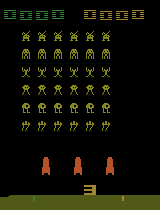
\includegraphics[width=0.8cm]{./imgs/si0.png}};
		\node [image, xshift=-0.1cm, yshift=0.1cm, opacity=0.6] at (frames)
			{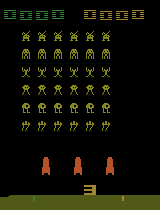
\includegraphics[width=0.8cm]{./imgs/si0.png}};
		\node [image] at (frames)
			{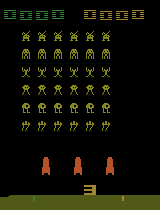
\includegraphics[width=0.8cm]{./imgs/si0.png}};
		%
		\begin{pgfonlayer}{below}
			\node [fit=(play) (train), box=orange, tight, opacity=0.5] {};
		\end{pgfonlayer}
	\end{tikzpicture}
	} \\[1.5cm]
	\subfloat[][Training a restrained agent.] {
	\begin{tikzpicture}
		\node (rb) [command text] {
			atarieyes features rb {\normalfont <features-file>} --stream
		};
		\node (train) [command text, below=1.5cm of rb] {
			atarieyes agent train --env {\normalfont <env-name>} --rb
		};
		\draw [flow] ([xshift=-2cm]train.north) --
			node (mid) [midway] {} ([xshift=-2cm]rb.south);
		\node [anchor=east, outer sep=1ex] at (mid) {$\bvec{o}_t$};
		\coordinate (frames) at ($(mid) + (1,0)$);
		\node [image, xshift=-0.2cm, yshift=0.2cm, opacity=0.3] at (frames)
			{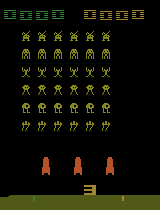
\includegraphics[width=0.8cm]{./imgs/si0.png}};
		\node [image, xshift=-0.1cm, yshift=0.1cm, opacity=0.6] at (frames)
			{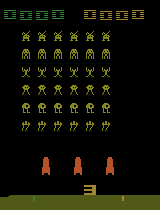
\includegraphics[width=0.8cm]{./imgs/si0.png}};
		\node [image] at (frames)
			{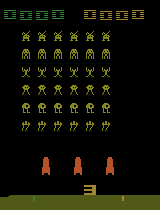
\includegraphics[width=0.8cm]{./imgs/si0.png}};
		\draw [flow] ([xshift=2cm]rb.south) --
			node [anchor=west, outer sep=1ex] {$(\vec{q}_t, r_t')$}
			([xshift=2cm]train.north);
		%
		\begin{pgfonlayer}{below}
			\node [fit=(rb) (train), box=blue!50!lightgray, tight, opacity=0.5] {};
		\end{pgfonlayer}
	\end{tikzpicture}
	} \\[1.5cm]
	\subfloat[][Training a new features extractor from a restrained agent.] {
	\begin{tikzpicture}
		\node (rb) [command text] {
			atarieyes features rb {\normalfont <features-file>} --stream
		};
		\node (play) [command text, below=1.5cm of rb] {
			atarieyes agent play {\normalfont <agent-file>} --rb --watch stream
		};
		\node (train) [command text, below=1.5cm of play] {
			atarieyes features train --env {\normalfont <env-name>}
		};
		\draw [flow] ([xshift=-2cm]play.north) --
			node (mid) [midway] {} ([xshift=-2cm]rb.south);
		\node [anchor=east, outer sep=1ex] at (mid) {$\bvec{o}_t$};
		\coordinate (frames) at ($(mid) + (1,0)$);
		\node [image, xshift=-0.2cm, yshift=0.2cm, opacity=0.3] at (frames)
			{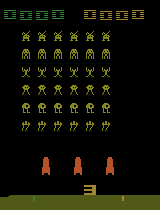
\includegraphics[width=0.8cm]{./imgs/si0.png}};
		\node [image, xshift=-0.1cm, yshift=0.1cm, opacity=0.6] at (frames)
			{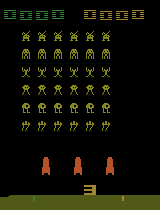
\includegraphics[width=0.8cm]{./imgs/si0.png}};
		\node [image] at (frames)
			{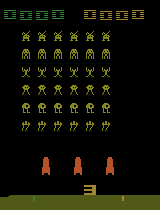
\includegraphics[width=0.8cm]{./imgs/si0.png}};
		\draw [flow] ([xshift=2cm]rb.south) --
			node [anchor=west, outer sep=1ex] {$(\vec{q}_t, r_t')$}
			([xshift=2cm]play.north);
		%
		\draw [flow] (play) -- node (mid1) [midway] {} (train);
		\coordinate (frames) at ($(mid1) + (1,0)$);
		\node [anchor=east, outer sep=1ex] at (mid1) {$\bvec{o}_t$};
		\node [image, xshift=-0.2cm, yshift=0.2cm, opacity=0.3] at (frames)
			{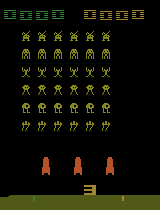
\includegraphics[width=0.8cm]{./imgs/si0.png}};
		\node [image, xshift=-0.1cm, yshift=0.1cm, opacity=0.6] at (frames)
			{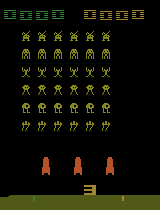
\includegraphics[width=0.8cm]{./imgs/si0.png}};
		\node [image] at (frames)
			{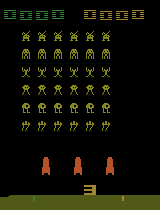
\includegraphics[width=0.8cm]{./imgs/si0.png}};
		%
		\begin{pgfonlayer}{below}
			\node [fit=(play) (train), box=orange, tight, opacity=0.5] {};
			\node [fit=(rb) (play), box=blue!50!lightgray, tight,
				opacity=0.5] {};
		\end{pgfonlayer}
	\end{tikzpicture}
	}
	\caption{How the various instances interact in each case.}
	\label{fig:cmd-instances}
\end{figure}

These instances use sockets to exchange observations, states and rewards. The
reason for this complete separation is that the main purpose of the
\texttt{atarieyes} package is to implement the Restraining Bolt and the
features extractor of Chapter~\ref{ch:fluents}, not a RL agent. In fact, there
are many modern and stable libraries implementing Deep RL agents. Thanks to
this separation, we can substitute \texttt{atarieyes agent} commands with any
software implementing a Deep RL agent. We don't need to restrict ourselves to
our implementation, not even to Double DQN. In fact, it's sufficient that the
agent's instance respects the interface of the socket messages. Since we also
provide Client--Server classes, the integration should be immediate.


\subsubsection*{Output}

To conclude this overview of the user interface, we look at the output of the 
various commands. As we've seen from \texttt{select}, the definitions for each
environment are stored in JSON files inside the \texttt{definitions/}
directory. Training commands, instead, store their result inside
\texttt{runs/}. For example,
\verb|atarieyes agent train -e Pong-v4| 
generates the following directories:
\begin{lstlisting}
runs/agent/Pong-v4/logs/0/
runs/agent/Pong-v4/models/0/
\end{lstlisting}
Every training generates ``logs'' and ``models'' directories in
unique paths composed with increasing numbers. In the example above, a new
output would be saved \verb|logs/1| and \verb|models/1|.

Inside the ``models'' directory we can find all the checkpoints saved
during training. These files can be passed as arguments to a \verb|--continue|
option, to load a saved agent. ``logs'' directory, instead, contains
\verb|args.json| and a file of TensorBoard logs. The JSON of arguments
\verb|args.json| is used for the \texttt{play} command or for the
\verb|--from| option, if we want to repeat a similar training.

The remaining files in the logs directory contain various metrics that allow
to follow the training process. These logs can be visualized with TensorBoard,
the TensorFlow visualization tool. In the example, we would run:
\begin{lstlisting}[style=bash]
poetry run tensorboard --logdir runs/agent/Pong-v4/logs/
\end{lstlisting}
For each episode, we can read: the number of steps, the cumulative reward, the
distribution of RB states, the distribution of selected actions, and other
metrics related to DQN.

The output of a \texttt{features train} command is really similar to that for
the agent: ``logs'' and ``models'' directories are saved under
\verb|runs/features| that contain the JSON of arguments, checkpoint files, and
TensorBoard logs. Intead, the main difference is the content of the log files.
Some informations that we save and can be visualized are the following:
\begin{description}
	\item [Scalar metrics] These are relevant scalar quantities that allow to
		follow the training algorithm. For RBM training, we store: free energy,
		reconstruction error, sparsity and normalization loss, learning rate.
		Instead, for the Boolean functions, we can read: average and maximum
		values of the sensitivity, consistency metrics, and fitness.
	\item [Images] Reconstructed most probable input images.
	\item [Graph] We can inspect the graph of computation of each step of the
		training algorithm. Each inner model of the features extractor has a
		different training graph. For the Boolean functions, for example, we
		observe the four steps of the genetic algorithm.
	\item [Distribution] We can observe how the model parameters are distributed
		on the real axis. This helps to investigate under/over-fitting and other
		issues. For the genetic algorithm we visualize the population fitness
		values, a projected representation of the individuals, and the fluents
		predictions.
\end{description}


\section{Implementation}

\label{sec:implementation}

The package has a modular and comprehensible design, as we can see from the
following file structure: \\[1ex]
\hspace{2ex}
\begin{minipage}[t]{0.25\textwidth}
	\begin{forest}
		dirtree
		[atarieyes/,baseline
			[\_\_main\_\_]
			[tools]
			[streaming]
			[layers]
			[automata]
		]
	\end{forest}
\end{minipage}
\hfill
\begin{minipage}[t]{0.25\textwidth}
	\begin{forest}
		dirtree
		[atarieyes/,baseline
			[agent/
				[training]
				[playing]
				[models]
			]
		]
	\end{forest}
\end{minipage}
\hfill
\begin{minipage}[t]{0.25\textwidth}
	\begin{forest}
		dirtree
		[atarieyes/,baseline
			[features/
				[training]
				[rb]
				[models]
				[genetic]
				[temporal]
				[selector]
			]
		]
	\end{forest}
\end{minipage}
\vspace{2ex}

\noindent
Each of these files is an importable Python module (extension omitted), with a
separate functionality. We won't discuss all of them, as we only want to look
at the most interesting details of the software.


\subsection{\texttt{atarieyes} package}

There are 5 modules inside the outer scope (left column of the file hierarchy
above). \verb|__main__.py| only realizes the command line interface and
\verb|tools.py| contains generic utilities. Instead, the remaining modules are
the most interesting.


\subsubsection*{\texttt{streaming} module}

This module allows the various instances of the program to communicate. It
defines a communication protocol and the format of the messages to exchange.
The program communicates through sockets. So, the RL agent and the Restraining
Bolt could even be on separate machines. Furthermore, this allows our
implementation of the features extractor and the Restraining Bolt to
communicate with any kind of RL agent, even implemented with some other
library. It's sufficient that the agent program does
\lstinline[style=inlinepy]|import atarieyes.streaming| to use this module
interface for exchanging messages with the Restraining Bolt.

This file defines two base classes: \texttt{Sender} and \texttt{Receiver}.
The sender is a TCP server that waits the incoming connection from the
receiver. They realize the basic functionality. Instead, the specific messages
format is defined in subclasses.

\texttt{AtariFramesSender} and \texttt{AtariFramesReceiver} is a pair of
subclasses that are used to send images of the Atari games, when the
\verb|--stream| option is present. Similarly, \texttt{StateRewardSender} and
\texttt{StateRewardReceiver} transmit the pair $(\vec{q}, r')$ of automaton
state and reward from the RB back to the agent.

The base classes provide transmit and receive buffers for an asynchronous
exchange. Users can send and receive data with \texttt{send} and
\texttt{receive} methods of the respective classes.


\subsubsection*{\texttt{automata} module}

The final layer of the features extractor model is composed by an array of
Boolean functions. As we've seen, this part is trained with a Genetic
Algorithm, which is essentially a stochastic search. This requires to maintain
a population of candidates and check all of them against the temporal
constraint. To do so, we continuously predict the fluents values with each
candidate. Then, after the 

Since the population can contain thousands of candidates, we implemented a



\subsection{\texttt{agent} package}

\label{sec:impl-agent}

% TODO: I've contributed to flloat

